\section*{Experimental setup}
To conduct the test with \textit{Transformed Up/Down Method} a program in MatLab was constructed. A flowchart over the program can be seen in \autoref{app:Flowchart} and the script for the program can be seen in \autoref{app:Script}. Other equiptment used in the experimental setup is a pair of Bang $\&$ Olufsen H6 headphones and a Lenovo Thinkpad with a fixed 10 \% volume.

Two tones are presented to the subject. After listening to the two tones the test subject chooses which of the two tones he or she believes to have the highest pitch. The subject chooses by typing either 1 (for the first presented tone) or 2 (for the last presented tone) in the command window (evt figur). 

The experiment was conducted in roomnumber B2-207 located on the 1st floor of Fredrik Bajers vej 7B at Aalborg University. On \autoref{fig:experiment} the experimental setup is illustrated. 

%\begin{figure}[H]
%\centering
%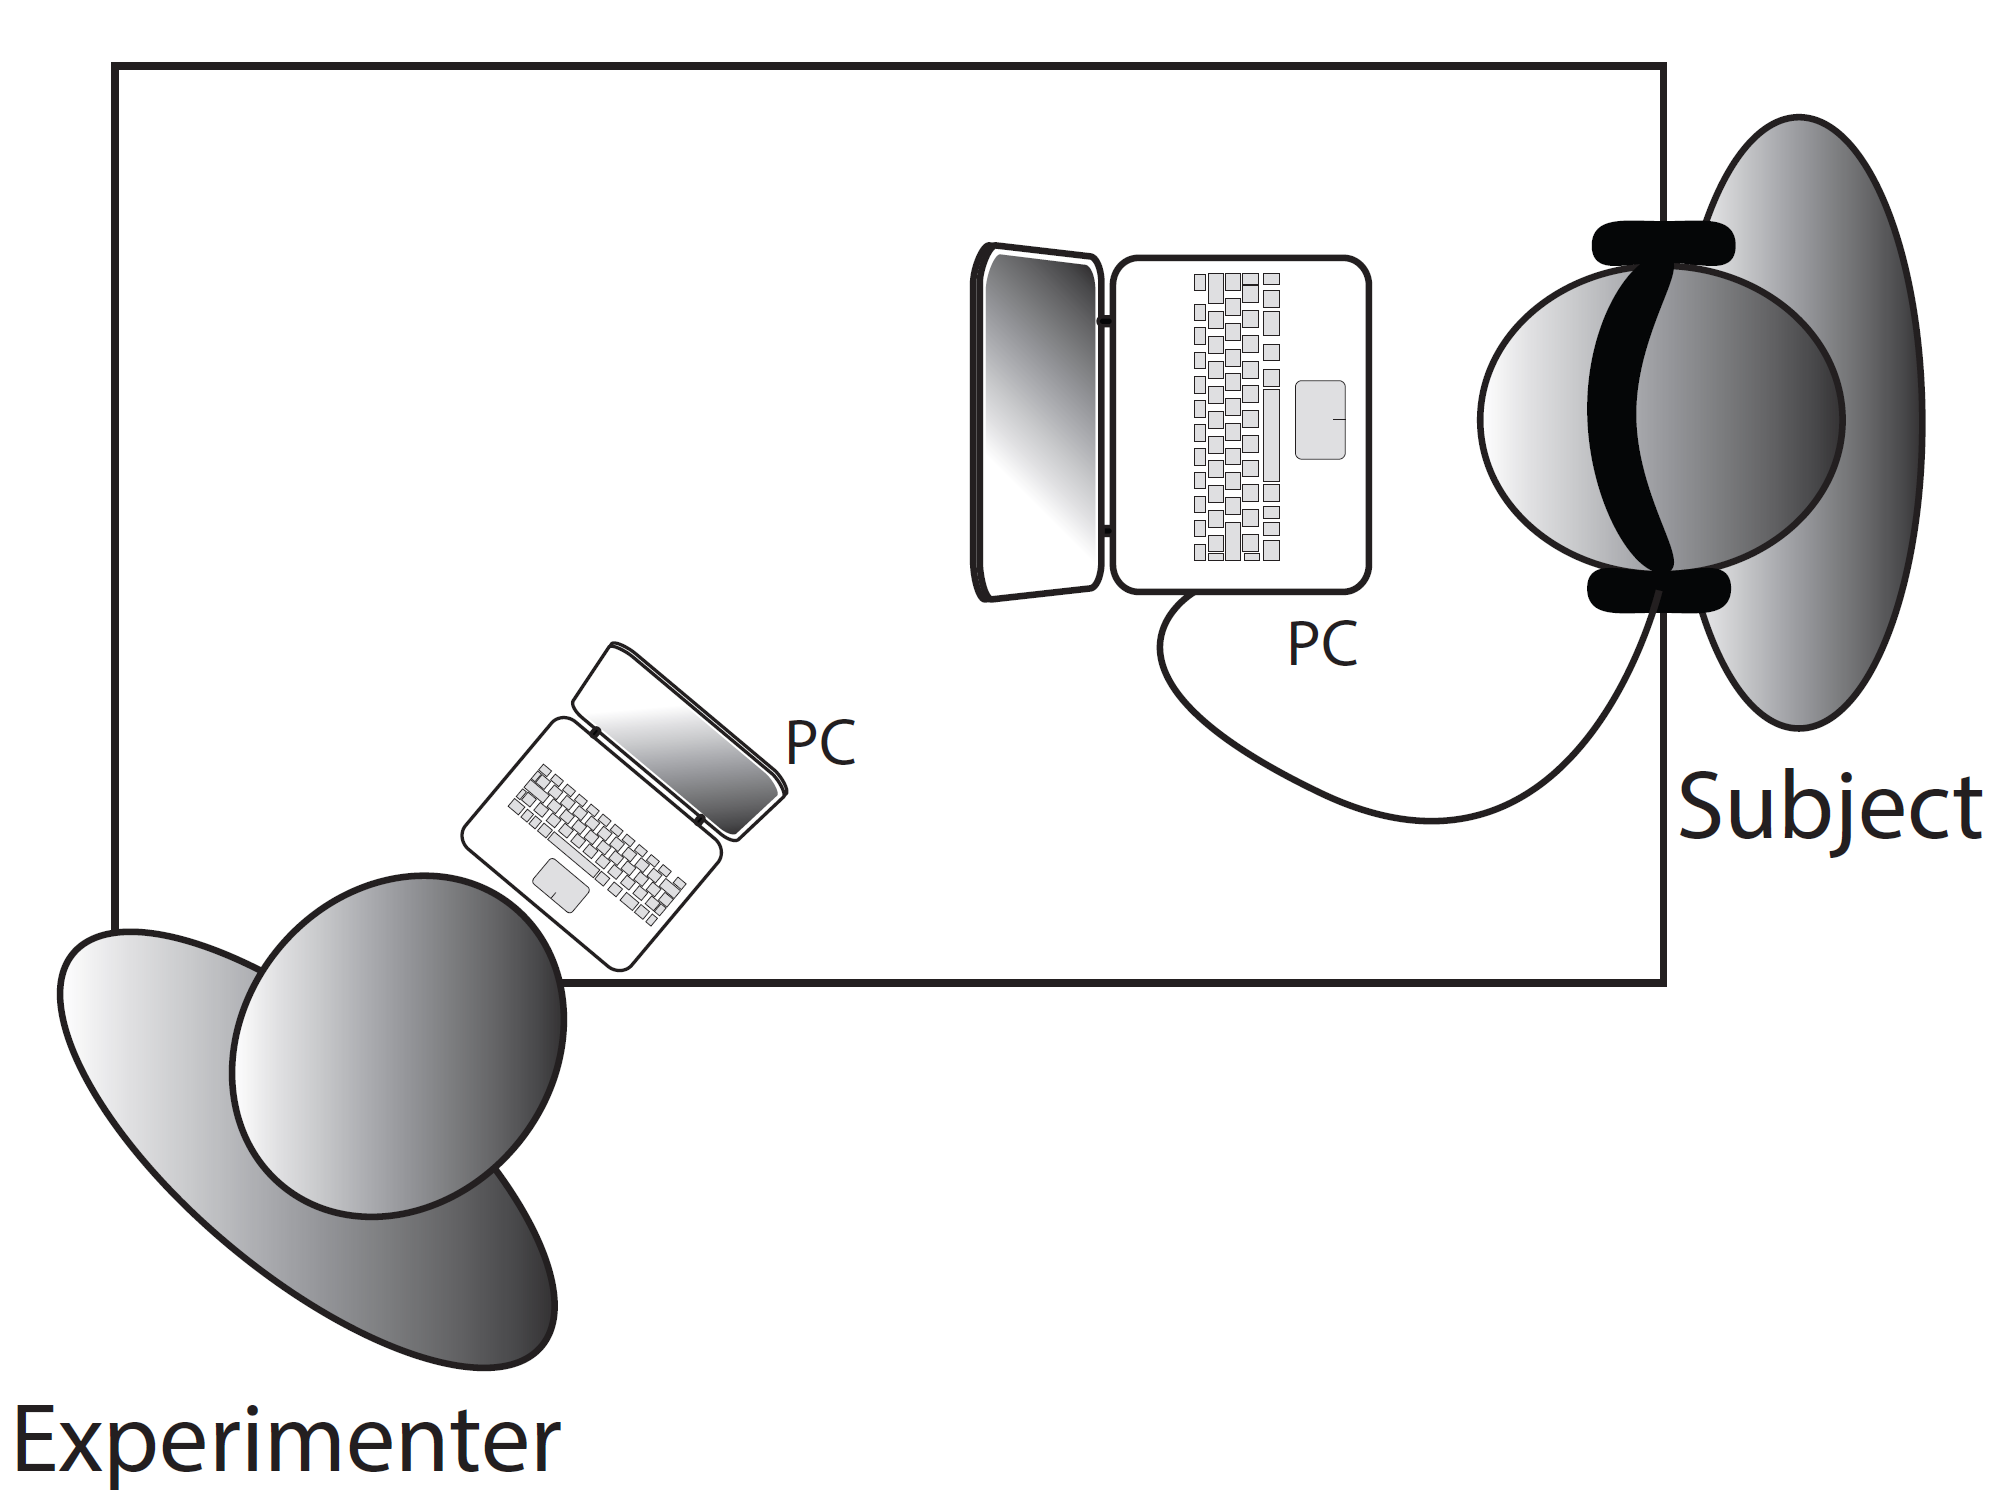
\includegraphics[width = 0.5\textwidth]{Figure/Vores_Figurer/experiment.png} 
%\caption{A sketch of the experimental setup}
%\label{fig:experiment}
%\end{figure}

\subsection*{Test subjects}
Five test subjects were used in the test. The subjects are two males and three females in the age of 23 to 24 (mean = 23.4). All of the test subjects are Enginerring Psychology students at Aalborg University. 